\documentclass[]{article}

\usepackage{amssymb}
\usepackage{booktabs}
\usepackage{listings}
\usepackage{hyperref}
\usepackage{cleveref}
\usepackage{graphicx}
\usepackage{tabularx}
%opening
\title{Extracting Greenhouse Gas Emission Values from Corporate Sustainability Reports\\
\large A Case Study on Evaluating and Finetuning Language Models on Long-Context Structured Information Extraction}
\date{February 1, 2024}

\begin{document}

\maketitle


\begin{abstract}
Information about greenhouse gas emissions by corporations is useful for a variety of purposes. However, this information is not published in a machine-readable format. Interested actors have to manually extract this information from sustainability reports. To solve this, a retrieval-augmented generation (RAG) system is developed to use language models for the long-context task of extracting scope 1, 2 and 3 emission data from sustainability reports. Furthermore, since ground truth data about this task is not publicly available, a dataset of sustainability reports and manually-extracted emission values ($N=100$) is collected. The collected data and developed system is used to evaluate a selection of language models, with Mixtral-8x7B-Instruct-v0.1 performing the best overall.

Using this information, a synthetic finetuning dataset is created using 3233 sustainability reports and emission data extracted by Mixtral-8x7B-Instruct-v0.1. Finetuning a LoRA for the significantly smaller Mistral-7B-Instruct-v0.2 on this dataset leads to a model that nearly reaches the performance of Mixtral-8x7B-Instruct-v0.1 on emission value extraction with an accuracy of 65\% (up from 46\% of the base model) and exceeds its performance on source page citation with an accuracy of 77\% (base model: 53\%), while being only a sixth of its size.

The findings of this work provide general indications on using language models for long-context structured information extraction tasks. The source code, data and models created in this project are open-sourced at \url{https://github.com/nopperl/corporate_emission_reports}.
\end{abstract}



\section{Problem Statement}
\label{sec:introduction}
Information about greenhouse gas emissions by corporations is useful for a variety of actors including journalists, policymakers and civil society. The importance of this information is underlined by the adoption of the Corporate Sustainability Reporting Directive \footnote{\url{https://eur-lex.europa.eu/legal-content/EN/TXT/?uri=CELEX:32022L2464}}, which requires EU companies to publish this information as part of sustainability reports starting with 2025. However, these reports are usually published as PDF documents and not machine-readable. Hence, emission information has to be extracted manually, which is a tedious and time-consuming task. To solve this problem, the aim of this project is to develop and evaluate a machine learning system to automatically extract this information from sustainability reports. The output can then be easily used by interested actors for further data analysis, e.g. as foundation for media reporting on climate change.

Furthermore, to evaluate this system and to encourage research into solving such a task, a dataset of sustainability reports and manually-extracted emission values is created and published.

As the dataset and system should be publically-accessible and inspectable, the focus of this project is on open-source models and software and the code and dataset are published at \url{https://github.com/nopperl/corporate_emission_reports}.

\subsection{Research objective}
The main result is a machine learning system which, given a sustainability report, extracts the Scope 1, 2 and 3 greenhouse gas emissions in metric tonnes of CO2eq in a machine-readable format. For the purpose of this project, the following definitions from the GHG Protocol Corporate Standard\footnote{\url{https://ghgprotocol.org/corporate-standard}} are used:

\begin{itemize}
	\item Scope 1: A reporting organization’s direct GHG emissions.
	\item Scope 2: A reporting organization’s emissions associated with the generation of electricity, heating/cooling, or steam purchased for own consumption.
	\item Scope 3: A reporting organization’s indirect emissions other than those covered in scope 2.
\end{itemize}

Note, that for scope 2 emissions, the market-based calculation is given precedence.

Furthermore, the system indicates if this data is missing from the report. To aid interpretability, the system also cites the parts of the input report referenced during extraction.

The second result is a dataset of corporate sustainability reports with manually-extracted emission values, which can be used to benchmark and evaluate automatic extraction systems.

The third result is an evaluation of the performance of the developed system using different language models based on the collected dataset.

\section{Dataset}
\label{sec:dataset}
To develop and evaluate the intended information extraction system, a gold standard dataset of corporate sustainability reports and their associated scope 1, 2 and 3 emissions is created. Since there is no publicly-available self-reported greenhouse gas emissions dataset, these values have to be manually extracted from the sustainability reports. Hence, the dataset is restricted to a small size of $N=100$, which is not large enough for training or finetuning models, but suffices for evaluation. For simplicity, only reports in English are considered. Note that sustainability reports based on the Carbon Disclosure Project \footnote{\url{https://www.cdp.net/en/guidance}} or Global Reporting Initiative \footnote{\url{https://www.globalreporting.org/standards/}} templates are not considered in order not to overfit to a specific format.

To ensure geographic diversity, three sets of companies headquartered on different continents are considered for the dataset. The first set consists of 39 corporations tracked by the Euro Stoxx 50 stock index as of 18 September 2023. Note that out of the missing 11 corporations of Euro Stoxx 50, 5 are not considered as no publicly-available sustainability reports were found and 6 are not considered as the author of this project was unable to extract unambiguous emission values. The second set is a random selection of 39 corporations listed on the New York Stock Exchange as of December 2023. The third set is a random selection of 22 corporations tracked by the Nikkei 225 index as of October 2023. Note, that this selection strategy is intentionally biased towards larger corporations due to the assumption that they have a higher likelihood of publishing sustainability reports.

For every corporation, the most recent sustainability report is downloaded from the official source. In some cases, the sustainability report is part of a larger annual report. The following information is manually extracted by the author of this project:

\begin{itemize}
	\item Scope 1 emissions in metric tonnes of CO2eq
	\item Scope 2 emissions in metric tonnes of CO2eq
	\item Scope 3 emissions in metric tonnes of CO2eq
	\item List of pages containing Scope 1 data
	\item List of pages containing Scope 2 data
	\item List of pages containing Scope 3 data
\end{itemize}

If the data does not exist in the report or cannot be unambiguously extracted, it is noted as missing.

Furthermore, additional data of potential use for future projects is extracted. These consists of:

\begin{itemize}
	\item Year of the most recent emission data
	\item Emissions for each of the 15 scope 3 categories \footnote{\url{https://ghgprotocol.org/scope-3-calculation-guidance-2}} in metric tonnes of CO2eq
	\item Report URL
	\item SHA-256 hash of the report PDF
\end{itemize}

\section{System}
\label{sec:method}

The system to automatically extract emission values from sustainability reports consists of four parts: The \emph{input data} (i.e., a sustainability report), which is inserted into a \emph{prompt}, which is used by a \emph{language model} to produce an \emph{output} (i.e., the structured emission data).

\subsection{Model}

The backbone of this system is the machine-learning model. Due to their versatility, decoder-only generative language models are suited for this task. Since the focus of this project is on open source models, proprietary models such as the state-of-the-art GPT-4 \cite{DBLP:journals/corr/abs-2303-08774} are not considered.

There are usually three types of models: base models, finetuned models and aligned models. Base models are simply trained on a large dataset of diverse texts. These base models can then be tailored for instruction-following tasked by supervised fine-tuning (SFT) on a smaller instruction dataset. Even further, these models can then be aligned to human preference using direct preference optimization (DPO) \cite{DBLP:conf/nips/RafailovSMMEF23} or reinforcement learning through human feedback. Since the instruction following capability is important to achieve the task, only instruction-following models are considered.


\begin{table}[]
	\begin{tabular}{lcc}
		\toprule
		\textbf{Model} & \textbf{Param Size} & \textbf{Context Length} \\ \midrule
		\href{https://huggingface.co/mistralai/Mistral-7B-Instruct-v0.2}{Mistral-7B-Instruct-v0.2} \cite{DBLP:journals/corr/abs-2310-06825} & 7B & 32768 \\
		\href{https://huggingface.co/openchat/openchat-3.5-0106}{openchat-3.5-0106} \cite{DBLP:journals/corr/abs-2309-11235} & 7B & 8192 \\
		\href{https://huggingface.co/Qwen/Qwen-1_8B-Chat}{Qwen-1.8B-Chat} \cite{qwen} & 1.8B & 8192 \\ 
		\href{https://huggingface.co/mistralai/Mixtral-8x7B-Instruct-v0.1}{Mixtral-8x7B-Instruct-v0.1} & 45B & 32768 \\ 
		\href{https://huggingface.co/miqudev/miqu-1-70b}{miqu-1-70b} & 70B & 32764 \\ \bottomrule
	\end{tabular}
	\caption{Language models used for the extraction task.}
	\label{tab:models}
\end{table}

\Cref{tab:models} gives an overview of the language models used in this project. Out of the \emph{small} class of language models consisting of 7 billion parameters or lower, Mistral can be considered state-of-the-art with its remarkable general performance \cite{DBLP:journals/corr/abs-2310-06825}. Note, that the instruction-tuned version of Mistral is used.

Keep in mind that language models are trained on a maximum sequence length, also known as context size. Mistral is trained for an unusually large context size of 32768 tokens. Since the task contains long input reports, this makes Mistral uniquely suited. Preliminary tests using different models with a context size of 2048 or 4096 showed significantly worse performance.

In order to investigate how much a larger training context size affects performance, the openchat model is used as alternative in the 7b class. While it was trained with a sequence length of only 8192 tokens, using the recent self-extend technique \cite{DBLP:journals/corr/abs-2401-01325} it might be competitive with Mistral on the studied task.

Furthermore, to investigate how large the parameter size needs to be for this task, the significantly smaller Qwen-1.8B model is also evaluated. Similarly to openchat-3.5-0106, this model was trained with a sequence length of 8192 tokens and requires the self-extend technique to work.

To ascertain the upper limit, the significantly larger Mixtral and miqu are also evaluated. These two models are selected is used as they performed significantly better than other $\geq45$B models in preliminary experiments, likely due to their larger context size.

All models are run using the llama.cpp \footnote{\url{https://github.com/ggerganov/llama.cpp}} inference engine.

\subsection{Input}

The input data consists of a sustainability report. While the report is in PDF format, language models operate on plain text. Hence, a plain-text XHTML representation of the PDF document is extracted using PyMuPDF \footnote{\url{https://pymupdf.readthedocs.io/en/latest/index.html}}. Importantly, images are stripped from this representation. While it is also possible to purely extract text content using PyMuPDF, the XHTML representation is chosen as it preserves some logical structure of the PDF document. An important example of this are footnotes, which can be placed right next to the emission values and thus make it impossible for the model to discern the correct value.

As sustainability reports are usually longer than a few pages, the entirety of their text does not fit into the context of language models. This problem is solved using retrieval-augmented generation (RAG) \cite{DBLP:conf/nips/LewisPPPKGKLYR020}. That is, the report is split into chunks and only chunks relevant to the input query are included in the generation prompt.

There are two important questions in RAG: how to split the input into chunks and how to find relevant chunks to the query. In this project, simple solutions are used for both. The input report is split into chunks by pages, i.e. every page is a chunk. An entire page is an unusually large chunk, but it represents a logical boundary that avoids the problem of smaller chunking leaving semantically associated information in different chunks.

The second task, i.e. finding relevant chunks, is usually done by embedding the chunks and input query into vector space using an embedding model such as UAE-Large-V1 \cite{li2023angle} and then selecting the chunks with the highest vector similarity. However, a simpler alternative is available in this project, as the relevant chunks contain the somewhat unique terms \texttt{Scope 1}, \texttt{Scope 2} and \texttt{Scope 3}. Simply selecting only chunks containing those terms is a crude but sufficient and fast solution.
%vector embeddings could be used instead or for reranking, but prelim tests showed not useful, as semantic ssim to numbers nmot there

\subsection{Prompt}
\label{subsec:prompt}
As the system uses general-purpose language models, a well-engineered prompt is crucial in order to produce the intended output. Furthermore, a good prompt is likely to boost the performance of the relatively small language models considered in this work.

An instruction-following prompt in ChatML format is used for this work, i.e. the prompt simulates a conversation between a user and an assistant and induces the model to assume the role of the assistant in its generation. It can be seen in \Cref{lst:prompt.simple} and is very detailed in order to prevent unintended outputs observed during development.

For every report, the instruction prompt is filled with the extracted chunks. Due to this, the model inputs reach a considerable length, as can be seen in \Cref{tab:token}. As this dangerously approaches (and sometimes even exceeds) the model context limits, promising but token-expensive prompting techniques such as chain-of-thought \cite{DBLP:conf/nips/Wei0SBIXCLZ22} or few-shot \cite{DBLP:conf/nips/BrownMRSKDNSSAA20} prompting can not be utilized.

\begin{table}[h]
	\begin{tabular}{lrrrr}
\toprule
 & max & mean & median & min \\
\midrule
token\_length & 60063.00 & 14544.31 & 12184.50 & 1004.00 \\
\bottomrule
\end{tabular}

	\caption{Statistics about the number of tokens in input prompts tokenized for the Mistral model.}
	\label{tab:token}
\end{table}


\subsection{Output}
In order to further process the extracted values, a consistent and machine-readable model output is crucial. To achieve this, the model will be prompted to respond with a JSON object using a specified schema. This output is enforced using llama.cpp's BNF grammar-based decoding and Pydantic type validation \footnote{\url{https://pydantic.dev}}.

\Cref{output.example} provides an example output extracted from the 2022 sustainability report by The Duckhorn Portfolio, Inc. \footnote{\url{https://www.duckhornportfolio.com/assets/client/File/BrandAssets/DWC/TDP_ESGReport-2022_FINAL.pdf}}. The relevant page 56 of the report can be seen in \Cref{fig:example.report.page}. The model outputs emission data using machine-readable numbers in a consistent unit. Furthermore, missing values are denoted using the \texttt{null} value. Additionally, the chunks used to arrive at the output are listed using their page number in the \texttt{sources} field. For interpretability purposes, a UI could convert these source ids into page numbers and display them to the user. Note, however, that the source ids in the output are not guaranteed to actually contain the emission values. To alleviate this, a UI could display all pages provided to the model in the prompt and highlight those referenced by the model in the output. Importantly, this field is restricted to a maximum of five numbers, as excessively long source lists defeat the purpose of this information.

\begin{lstlisting}[label=output.example,caption={Example output.}]
{"scope_1":581,"scope_2":1220,"scope_3":null,"sources":[16,17,56,7]}
\end{lstlisting}

\begin{figure}
	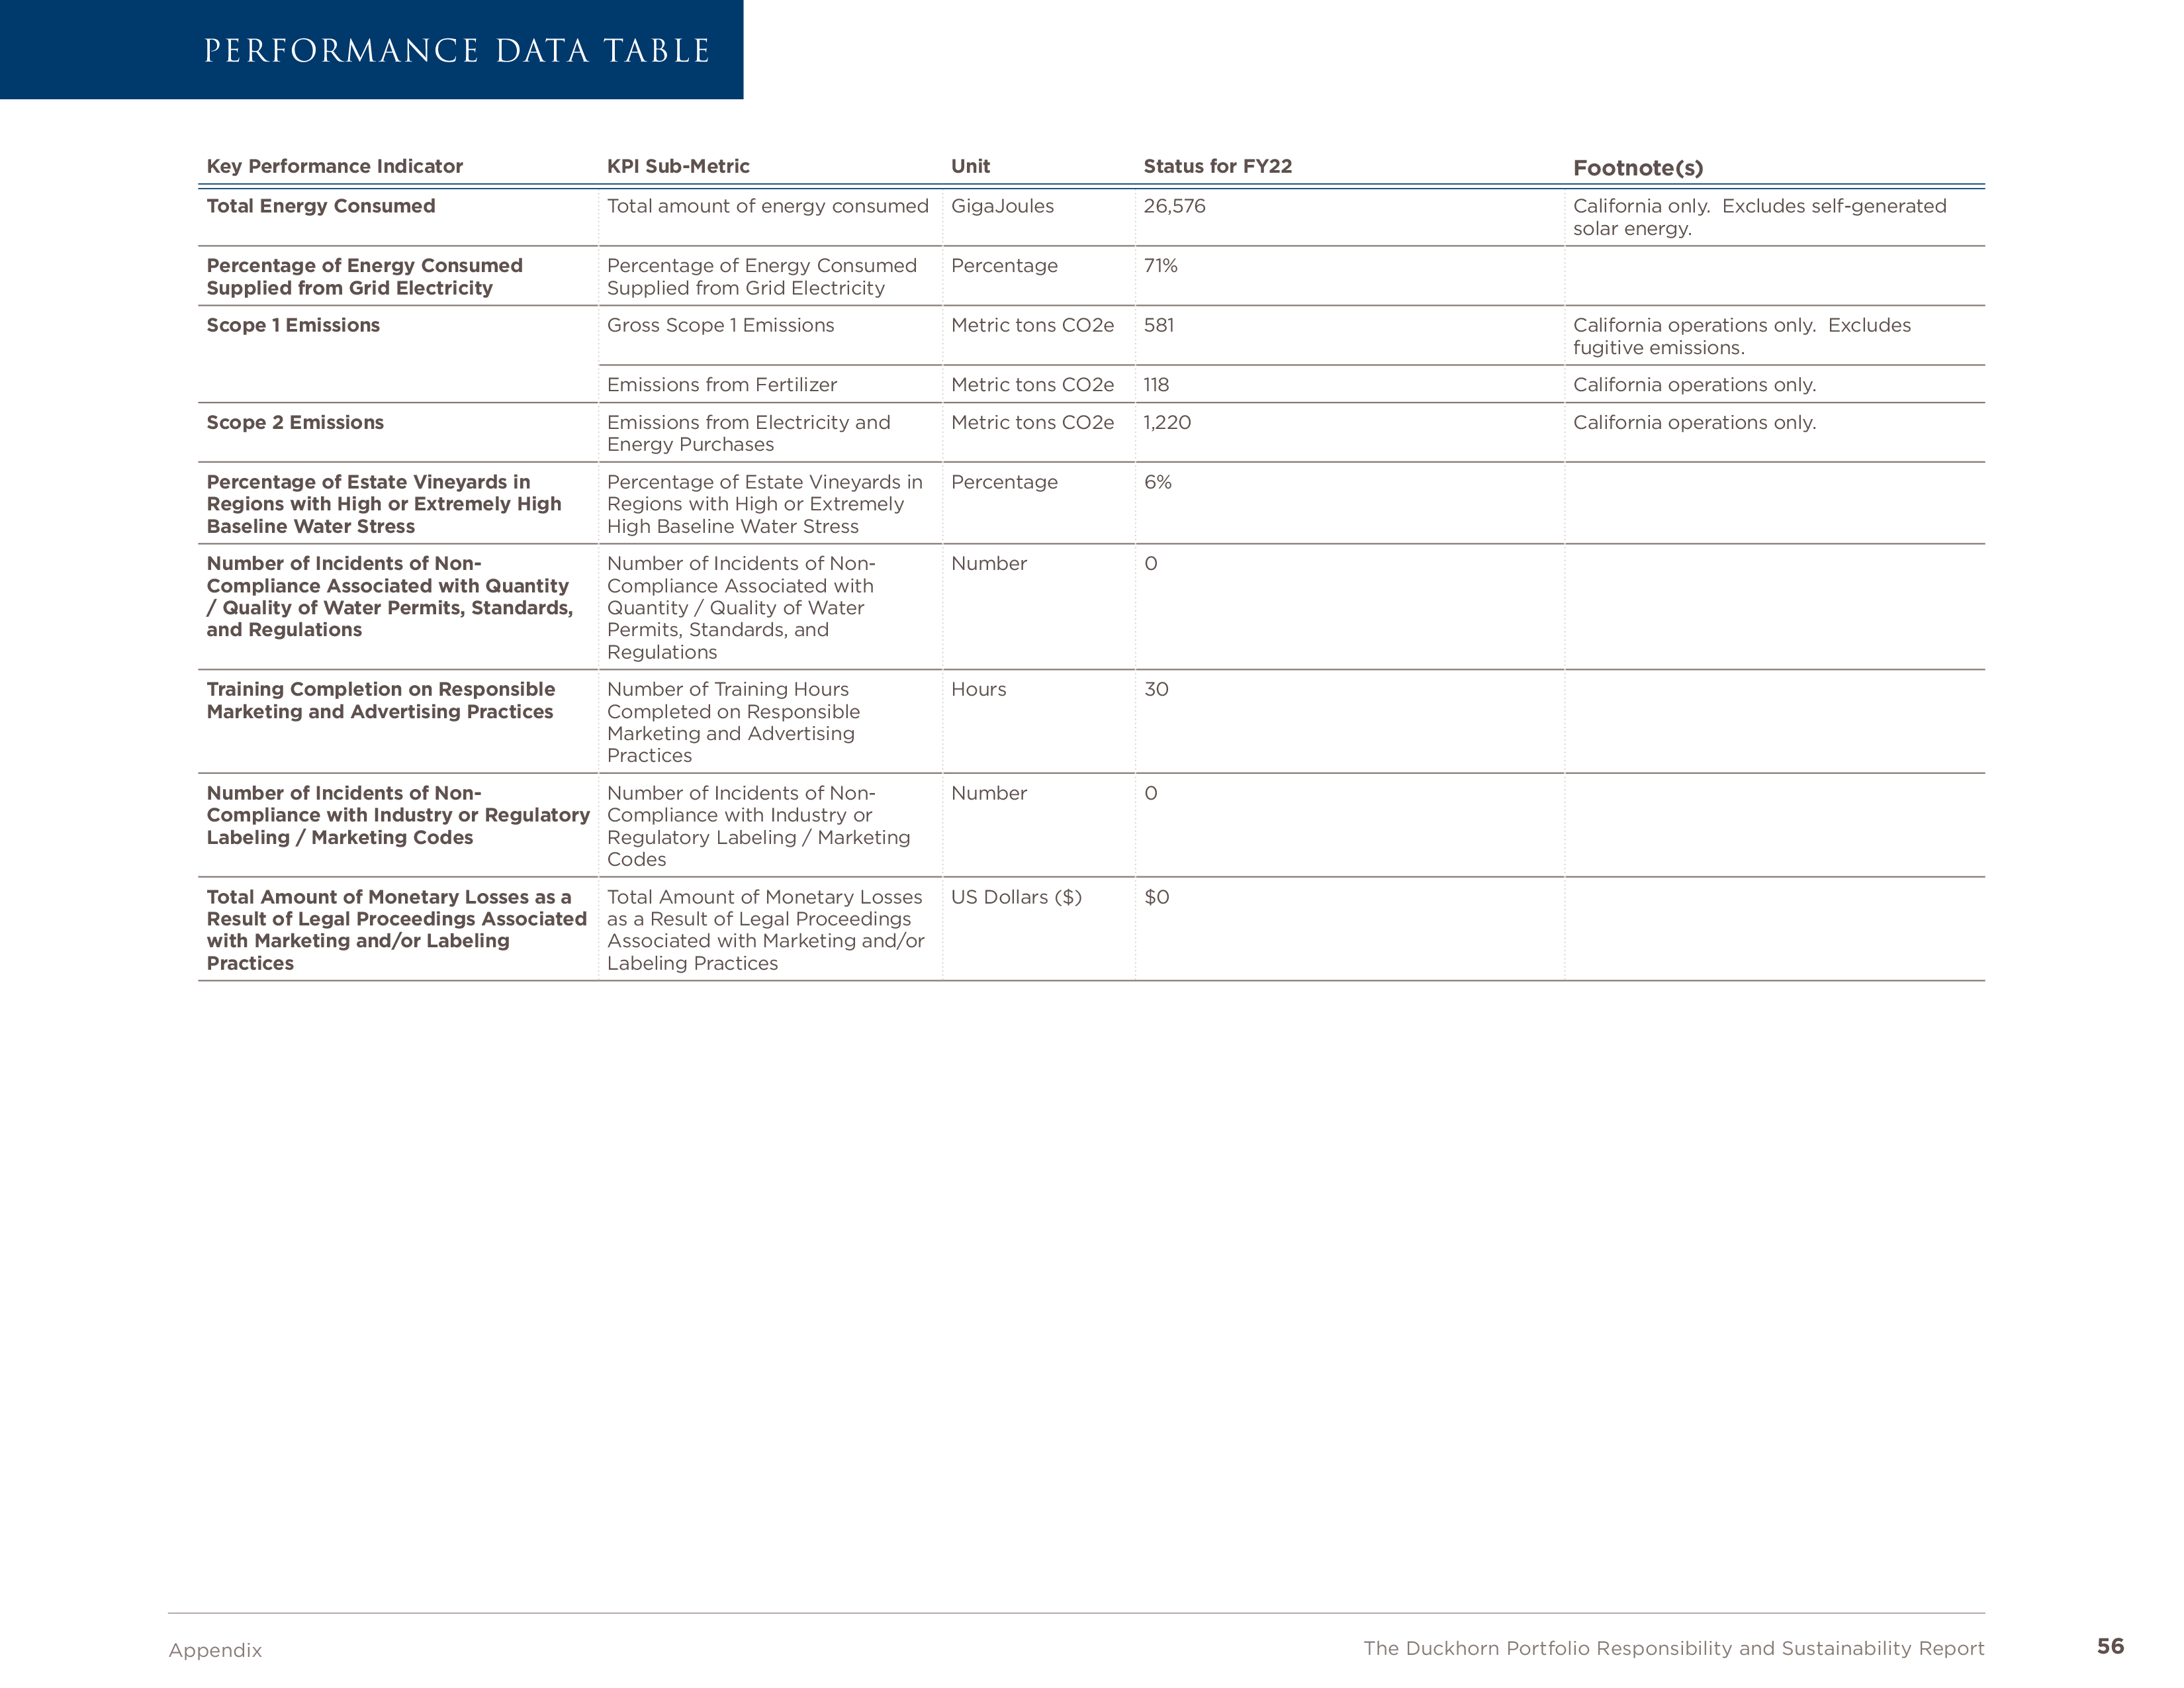
\includegraphics[width=\textwidth]{graphics/example-report-page}
	\caption{Relevant emission page of the 2022 sustainability report by The Duckhorn Portfolio, Inc.}
	\label{fig:example.report.page}
\end{figure}

\section{Evaluation}
\label{sec:eval}

The selected models in \Cref{tab:models} are evaluated using the manually-collected dataset of sustainability reports and associated emission values described in \Cref{sec:dataset} and the developed system described in \Cref{sec:method}. The evaluation serves as benchmark for the task motivated in \Cref{sec:introduction} as well as for the general use case of long-context structured information extraction.

\subsection{Setup}

The evaluation is run on a Linux system with an Nvidia GeForce RTX 2080 Ti GPU. Python 3.8.5 and CUDA 11.5.0 are used to run the experiments.

For the model comparison, all models are used in a consistent manner. The models are downloaded in the safetensors format\footnote{\url{https://huggingface.co/docs/safetensors/index}} and converted to the GGUF format with float16 data type using llama.cpp scripts.

Each model is run using the prompt as described in \Cref{subsec:prompt}. For models which were not trained using the ChatML format, the prompt is converted to the instruction format specified in their tokenizer configuration.

\subsection{Results}

	Performance is measured using two metrics:
	\begin{enumerate}
		\item accuracy for every extracted emission value
		\item source page retrieval accuracy
	\end{enumerate}
	
	\begin{table}[h!]
		\centering
		\begin{tabular}{@{}ccccccc@{}}
			\toprule
			scope 1 & scope 2 & scope 3 & avg of scopes & sources & model \\ \midrule
			49 & 34 & 54 & \textbf{46} & 53 & mistral \\
			33 & 31 & 56 & \textbf{40} & 48 & openchat \\
			12 & 8 & 5 & \textbf{8} & 3 & qwen-1.8B \\
			69 & 72 & 57 & \textbf{66} & 74 & miqu \\
			70 & 71 & 69 & \textbf{69} & 64 & mixtral \\
			65 & 62 & 69 & \textbf{65} & 77 & lora \\ \bottomrule
		\end{tabular}
		\caption{Performance comparison of different models}
		\label{tab:performance}
	\end{table}
	
	\Cref{tab:performance} shows that Mixtral significantly outperforms the smaller models. Out of the smaller models, Mistral performs the best. Qwen-1.8B-Chat does not yield good results, but it is still surprising that it is even able to produce relevant outputs for emission values (which similar models such as phi-2 or stablelm-zephyr-3b failed to do). The Mistral model finetuned on Mixtral outputs on a different dataset remarkably nearly matches or partially exceeds Mixtral, which is important, as a 7B model is far easier to deploy than a 45B model.
	
	It is notable that scope 2 accuracy is significantly lower for all models except Mixtral, likely due to oftentimes both market-based and location-based scope 2 emissions being present.
	
	\subsection{Numerical issues}
	
	Since language models struggle with numerical tasks, it is investigated whether wrong extractions are due to numerical errors instead of failures in logic. \Cref{tab:numerical_accuracy} shows the performance with accuracy measured by interpreting values within 10\% of each other as matching. All models significantly perform better using this metric, confirming that they stuggle with reproducing numbers correctly. Notably, this is also true for Mixtral.
	
	\begin{table}[h!]
		\centering
		\begin{tabular}{@{}cccccc@{}}
			\toprule
			scope 1 & scope 2 & scope 3 & avg of scopes & model \\ \midrule
			60 & 39 & 61 & \textbf{53} & mistral \\
			43 & 43 & 60 & \textbf{49} & openchat \\
			14 & 12 & 5 & \textbf{10} & qwen-1.8B \\
			78 & 75 & 71 & \textbf{75} & mixtral \\
			70 & 66 & 71 & \textbf{69} & lora \\ \bottomrule
		\end{tabular}
		\caption{Performance comparison using a 10\% margin for numerical accuracy}
		\label{tab:numerical_accuracy}
	\end{table}
	
	Furthermore, it is possible that extraction failures are due to wrong conversions of numbers into metric tons. This is investigated by computing accuracy irrespective of the unit. Again, the results in \Cref{tab:unit_agnostic_accuracy} show that the models perform better using this metric, confirming that they struggled with converting the numbers in the report to the correct unit.
	
	\begin{table}[h!]
		\centering
		\begin{tabular}{@{}cccccc@{}}
			\toprule
			scope 1 & scope 2 & scope 3 & avg of scopes & model \\ \midrule
			54 & 36 & 59 & \textbf{50} & mistral \\
			35 & 35 & 62 & \textbf{44} & openchat \\
			17 & 11 & 8 & \textbf{12} & qwen-1.8B \\
			76 & 83 & 76 & \textbf{78} & mixtral \\
			79 & 78 & 81 & \textbf{79} & lora \\ \bottomrule
		\end{tabular}
		\caption{Performance comparison using unit-agnostic accuracy}
		\label{tab:unit_agnostic_accuracy}
	\end{table}
	
	\subsection{Prompt engineering}
	
	\begin{table}[h!]
		\centering
		\begin{tabular}{@{}ccccccc@{}}
			\toprule
			scope 1 & scope 2 & scope 3 & avg of scopes & sources & model & type \\ \midrule
			38 & 31 & 44 & \textbf{38} & 52 & mistral & no starting answer \\
			49 & 34 & 54 & \textbf{46} & 53 & mistral & starting answer \\ \bottomrule
		\end{tabular}
		\caption{Comparison of default ChatML prompts and ChatML prompts with the assistant's answer already started}
		\label{tab:prompt_comparison}
	\end{table}
	
	Engineering good prompts is important to improve model performance. \Cref{tab:prompt_comparison} compares default ChatML prompts and ChatML prompts with the assistant's answer already started by: \texttt{I have extracted the Scope 1, 2 and 3 emission values from the document, converted them into metric tons and put them into the following json object: ```json}. The results clearly show that the latter prompt leads to a better performance.
	
	\subsection{Self-extend}
	
	\begin{table}[h!]
		\centering
		\begin{tabular}{@{}cccccccc@{}}
			\toprule
			scope 1 & scope 2 & scope 3 & avg of scopes & sources & failures & model & self-extend \\ \midrule
			40 & 32 & 50 & \textbf{41} & 30 & 40 & openchat & no \\
			33 & 31 & 56 & \textbf{40} & 48 & 4 & openchat & yes \\ \bottomrule
		\end{tabular}
		\caption{Evaluation of the usefulness of self-extend}
		\label{tab:self_extend}
	\end{table}
	
	The openchat model is used to evaluate the usefulness of self-extend. \Cref{tab:self_extend} shows that running the openchat model without self-extend failed for 40 out of 100 reports, while it failed only on 4 reports when using self-extend. These crashes occur for long input prompts. This strongly shows that self-extend is able to significantly extend the context size of the model.
	
	\subsection{Finetuning}
	\subsubsection{Overview}


\begin{table}[h]
	\centering
	\begin{tabular}{l|l|l|l|l|l|l|l|}
		\hline
		scope 1 & scope 2 & scope 3 & avg of scopes & sources & learning rate & epochs & type \\\hline
		49 & 34 & 54 & \textbf{46} & 53 & - & - & mistral \\\hline
		70 & 71 & 69 & \textbf{69} & 64 & - & - & mixtral \\\hline
		65 & 62 & 69 & \textbf{65} & 77 & 2e-5 & 3 & lora \\\hline
	\end{tabular}
	\caption{Performance comparison between base model and finetuned models using different techniques.}
	\label{tab:finetuning-comparison}
\end{table}

	To investigate whether the performance of Mixtral can be achieved by a smaller, easier to deploy model, the Mistral-7B model is finetuned by training a LoRA on a dataset of 3233 sustainability reports and emission values extracted by Mixtral for 3 epochs. The results in \Cref{tab:finetuning-comparison} show that the finetuned model not only significantly outperforms the base model, but remarkably nearly matches and partially exceeds the performance of Mixtral, at a much smaller size.


\subsubsection{DPO}

\begin{table}[h]
	\centering
	\begin{tabular}{|l|l|l|l|l|l|l|l|}
		\hline
		scope 1 & scope 2 & scope 3 & avg of scopes & sources & learning rate & epochs & type \\\hline
		49 & 34 & 54 & \textbf{46} & 53 & - & - & base \\\hline
		43 & 37 & 55 & \textbf{45} & 60 & 5e-6 & 1 & sft \\\hline
		32 & 32 & 49 & \textbf{38} & 58 & 5e-6 & 1 & dpo \\\hline
	\end{tabular}
	\caption{Performance comparison between base model and LoRA models finetuned using supervised learning and DPO.}
	\label{tab:dpo-comparison}
\end{table}

The LoRA was also trained using DPO \cite{DBLP:conf/nips/RafailovSMMEF23} by constructing a binary preferences dataset with randomly generated rejected outputs. \Cref{tab:dpo-comparison} shows that the model finetuned using DPO performs significantly worse than the one using supervised finetuning.

\subsubsection{Rank comparison}

\begin{table}[h]
	\centering
	\begin{tabular}{|l|l|l|l|l|l|l|l|}
		\hline
		scope 1 & scope 2 & scope 3 & avg of scopes & sources & learning rate & epochs & rank \\\hline
		38 & 35 & 47 & \textbf{40} & 59 & 5e-6 & 1 & 4 \\\hline
		43 & 37 & 55 & \textbf{45} & 60 & 5e-6 & 1 & 32 \\\hline
		42 & 37 & 54 & \textbf{44} & 59 & 5e-6 & 1 & 64 \\\hline
		56 & 38 & 57 & \textbf{47} & 56 & 5e-6 & 1 & 128 \\\hline
	\end{tabular}
	\caption{Performance comparison between LoRA models with different ranks.}
	\label{tab:rank-comparison}
\end{table}

An important hyperparameter for training LoRA's is the LoRA rank. \Cref{tab:rank-comparison} shows that a rank of 128 performed the best, with 32 performing the second-best. However, this is not as clear anymore when a different learning rate is used, as can be seen in \Cref{tab:rank-lr-comparison}. Therefore, a rank of 32 was used for all other training runs.

\begin{table}[h]
	\centering
	\begin{tabular}{|l|l|l|l|l|l|l|l|}
		\hline
		scope 1 & scope 2 & scope 3 & avg of scopes & sources & learning rate & epochs & rank \\\hline
		64 & 66 & 74 & \textbf{68} & 65 & 2e-5 & 1 & 32 \\\hline
		60 & 58 & 69 & \textbf{62} & 69 & 2e-5 & 1 & 128 \\\hline
	\end{tabular}
	\caption{Performance comparison between LoRA models with different ranks and learning rates.}
	\label{tab:rank-lr-comparison}
\end{table}

\subsubsection{Learning rate comparison}

As mentioned above, a learning rate of 2e-5 led to better results than 5e-6 both at epoch 1 and 3, as shown in \Cref{tab:lr-comparison}.

\begin{table}[h]
	\centering
	\begin{tabular}{|l|l|l|l|l|l|l|l|}
		\hline
		scope 1 & scope 2 & scope 3 & avg of scopes & sources & learning rate & epochs & rank \\\hline
		43 & 37 & 55 & \textbf{45} & 60 & 5e-6 & 1 & 32 \\\hline
		64 & 66 & 74 & \textbf{68} & 65 & 2e-5 & 1 & 32 \\\hline
		60 & 57 & 68 & \textbf{62} & 67 & 5e-6 & 3 & 32 \\\hline
		65 & 62 & 69 & \textbf{65} & 77 & 2e-5 & 3 & 32 \\\hline
	\end{tabular}
	\caption{Performance comparison between LoRA models with different learning rates.}
	\label{tab:lr-comparison}
\end{table}

\subsubsection{Epochs comparison}

It can be seen above that performance increases significantly from epoch 1 to 3 for a learning rate of 5e-6. \Cref{tab:epochs-lr-comparison} shows the case for a learning rate of 2e-5. Interestingly, scope 2 and 3 accuracy decreases after the first epoch, while source accuracy increases significantly. At epoch 4, all metrics except scope 1 accuracy decrease. On average, the performance at 3 epochs is slightly better, therefore this model is used.

\begin{table}[h]
	\centering
	\begin{tabular}{|l|l|l|l|l|}
		\hline
		scope 1 & scope 2 & scope 3 & avg of scopes & learning rate \\\hline
		64 & 66 & 74 & \textbf{68} & 2e-5 \\\hline
		65 & 62 & 69 & \textbf{65} & 2e-5 \\\hline
		67 & 59 & 68 & \textbf{65} & 2e-5 \\\hline
	\end{tabular}
	\caption{Performance comparison between LoRA models with different learning rates and epochs.}
	\label{tab:epochs-lr-comparison}
\end{table}

\subsubsection{Qwen-1.8B}

As the Qwen-1.8B model is even easier to deploy than Mistral-7B, it was also investigated whether finetuning it increases its performance to a sufficient level. Qwen1.5-1.8B-Chat was used as base model due to its better support. \Cref{tab:qwen-comparison} shows that the performance of the finetuned model is better, but still far from sufficient.

\begin{table}[h]
	\centering
	\begin{tabular}{|l|l|l|l|l|l|l|l|}
		\hline
		scope 1 & scope 2 & scope 3 & avg of scopes & sources & learning rate & epochs & type \\\hline
		12 & 8 & 5 & \textbf{8} & 3 & - & - & qwen-1.8B \\\hline
		3 & 5 & 22 & \textbf{10} & 6 & 2e-4 & 4 & qwen-1.8B lora \\\hline
	\end{tabular}
	\caption{Performance comparison between the base Qwen-1.8B model and the finetuned Qwen-1.8B model.}
	\label{tab:qwen-comparison}
\end{table}	
	
	\subsection{Additional Findings}
	
	
	Interestingly, different self-extend hyperparameters yielded the optimal performance for different models. \Cref{tab:self-extend-params} lists the used values. The neighbour size especially is unusually and counterintuitively high.
	
	\begin{table}[h!]
		\centering
			\begin{tabularx}{.5\textwidth}{ccc}
				\toprule
				model & neighbour size & group size \\
				\midrule
				mistral & 8 & 1024 \\
				mixtral & 8 & 1024 \\
				openchat & 16 & 2048 \\
				qwen & 64 & 2048 \\
				\bottomrule
			\end{tabularx}
			\caption{Self-extend hyperparameters used in the evaluation.}
			\label{tab:self-extend-params}
	\end{table}
	

\section{Conclusion}
Contributions of this project are:

	\begin{itemize}
	\item A manually-created evaluation dataset ($N=100$),
	\item a synthetic finetuning dataset ($N=3233$),
	\item an evaluation of multiple models (1.8B-45B) covering prompt strategies, numerical issues and self extend,
	\item an evaluation of different finetuning configurations,
	\item a finetuned Mistral-7B model which nearly matches and partially exceeds Mixtral (45B) on this task, and
	\item a web demo (\url{https://huggingface.co/spaces/nopperl/emission-extractor}).
\end{itemize}

Additionally, this work provided general indications on using language models for long-context structured information extraction tasks.

\subsection{Future Work}

Noting the limitations of the presented work, there are numerous ways for future improvements.

In this work, all extracted chunks of the report are input into the model in a single run, relying on the capability of the model to resolve ambiguities and connect information from multiple pages. However, in most reports, the relevant values are contained in a single page, even if it is duplicated on multiple pages. In other words, there are no intra-page information dependencies. Hence, it would probably be possible to prompt each page individually, with a final prompt on all page extractions leading to the final output for the whole report. This would require a smaller context size, which would enable token-expensive prompting techniques such as chain-of-thought \cite{DBLP:conf/nips/Wei0SBIXCLZ22} or few-shot \cite{DBLP:conf/nips/BrownMRSKDNSSAA20} prompting to be used. On the other hand, the system would have a longer runtime due to the necessity of running the model multiple times.

An important learning from collecting the dataset was that information is sometimes only displayed in graphs, which are not represented well in plain text form and require visual input to solve correctly. Multimodal (vision-language) models such as CogVLM \cite{DBLP:journals/corr/abs-2311-03079} might perform better on these reports.

Similarly, while the focus was on large decoder-only language models, it may be interesting to test how smaller encoder(-decoder) models such as (XLM-)RoBERTa or DeBERTa perform. These models could be finetuned on the Mixtral output dataset. However, the average input sequence is far longer than their context size.

Furthermore, since the collected dataset also includes values for all scope 3 emission categories, these data could be extracted by a future system.

\clearpage
\appendix
\section{Prompt}
\lstinputlisting[label=lst:prompt.simple,breaklines,caption={Simple instruction-following prompt.}]{../corporate_emission_reports/prompt-templates/simple.txt}


\bibliographystyle{plain}
\bibliography{bibliography}

\end{document}
